\chapter{Strutture dei Sistemi Operativi}
Analizziamo ora le regole e gli strumenti necessari per l'implementazione di un sistema operativo.

Esso è un sistema complesso, è quindi fondamentale definire correttamente i requisiti. Essi si possono definire da vari punti di vista: i servizi che dovrà fornire, l'interfaccia messa a disposizione agli utenti e ai programmatori.

\section{Servizi}

Alcune classi di servizi che il sistema operativo può fornire nei confronti dell'utente:
\begin{sitemize}
    \item \textbf{Interfaccia Utente:}

    Quasi tutti i sistemi operativi sono dotati di un'interfaccia utente, che può prendere molte forme diverse, la linea di comando, un'interfaccia grafica, ...

    Si può interagire con essa in molti modi, con mouse e tastiera, con uno schermo touch, ...

    \item \textbf{Esecuzione di Programmi:}

    Il sistema deve essere in grado di caricare un programma in memoria ed eseguirlo, inoltre deve essere in grado di rilevare e gestire situazioni di errore.

    \item \textbf{Operazioni I/O:}

    Il sistema operativo fornisce ai programmi dell'utente un modo per accedere ai dispositivi I/O.

    \item \textbf{Gestione del File-System:}

    I programmi utente devono essere in grado di creare, leggere, scrivere ed eliminare file e devono potersi muovere nella struttura dell'archiviazione.

    \item \textbf{Comunicazioni:}

    I programmi devono essere in grado di comunicare ad altri processi presenti sullo stesso sistema oppure ad altri sistemi connessi via rete.
    La comunicazione può essere implementata tramite memoria condivisa, oppure come scambio di messaggi

    \item \textbf{Rilevamento di Errori:}

    Il sistema operativo deve tenere sotto costante controllo CPU, memoria e dispositivi I/O per rilevare e gestire gli errori che sorgono durante l'esecuzione dei programmi utente.
\end{sitemize}

\spacer
Ci sono altri servizi che il sistema operativo deve eseguire per assicurarsi che il sistema funzioni in modo efficiente:

\begin{sitemize}
    \item \textbf{Allocazione di Risorse:}

    Quando ci sono più processi o più utenti diventa fondamentale gestire in modo efficiente le risorse hardware tra di essi, in particolare la CPU e la memoria.
    I dispositivi I/O spesso vengono gestiti in modo meno rigido utilizzando delle regole generali.

    \item \textbf{Logging:}

    Risolta essere importante registrare quali programmi e in quali quantità utilizzano le risorse del sistema.
    Queste statistiche sono preziose per gli amministratori che possono capire l'effettiva necessità di risorse.

    \item \textbf{Protezione e Sicurezza:}

    Ai possessori di informazioni su un sistema multiutente o distribuito deve essere garantito i propri dati da accessi indesiderati.

    La protezione riguarda il controllo di tutti gli accessi alle risorse di sistema.

    La sicurezza si basa sull'obbligo di autenticazione mediante password o sistema equivalente.
\end{sitemize}

\subsection{Interfaccia Utente}
Vista la sua importanza dal punto di vista dell'utente può essere utile approfondire le interfacce che permettono agli utenti di comunicare con il sistema operativo.

\subsubsection*{Command Line Interpreter (CLI)}

L'interfaccia a linea di comando permette di impartire comandi direttamente al sistema operativo.
Viene talvolta implementata dal kernel oppure attraverso programmi di sistema, inoltre può essere anche installata dall'utente, il sistema operativo può offrire più \textit{shell}.

\spacer
I comandi impartiti dall'utente possono essere eseguiti secondo due modalità:

\begin{sitemize}
    \item Se il codice del comando è relativo all'interprete viene chiamata direttamente la funzione richiesta dall'utente.

    \item Se invece il codice del comando viene implementato da un altro programma di sistema l'interprete utilizza il comando per accedere al file contenente il codice per l'esecuzione e lo inizializza.
\end{sitemize}

\begin{note}
    Spesso nei sistemi operativi non sono disponibili tutte le funzionalità tramite l'interfaccia grafica, in questi casi si può accedervi tramite l'interprete a linea di comando.

    \spacer[4pt]
    Inoltre la linea di comando risulta essere utile per l'esecuzione di comandi ripetuti in quanto è programmabile
\end{note}

\subsubsection*{Graphical User Interface (GUI)}

L'interfaccia grafica user-friendly realizza la metafora della scrivania (\textit{desktop}).

L'utente può muovere un cursore su icone che rappresentano programmi, file, cartelle e funzioni di sistema.

Questo rende semplice l'interazione con il sistema tramite mouse, tastiera e monitor.

\begin{note}
    L'interfaccia grafica nasce dal lavoro del centro di ricerca \textit{Xerox Palo Alto Research Center (PARC)}, le cui idee vennero poi riprese da Steve Jobs nella creazione del software per il primo Machintosh.

    \spacer[4pt]
    Gli sviluppatori di apple non hanno però mai avuto accesso al codice, quindi provarono ad ricrearlo partendo da una semplice dimostrazione, nella maggior parte delle situazioni riusciranno addirittura a migliorare le funzionalità del sistema della Xerox.

    \spacer[4pt]
    La storia ha un triste epilogo con la Xerox che provò a fare causa ad apple sul copyright dell'interfaccia, ma una corte statunitense porrà fine alla causa un anno dopo scagionando apple.
\end{note}

\section{Chiamate di Sistema}
Le chiamate di sistema forniscono un'interfaccia tra i programmi e i servizi offerti dal sistema operativo.

Questo permette al programmatore di chiamare le funzioni da linguaggi di programmazione ad alto livello (C o C++) anche se l'implementazione può essere stata fatta ad esempio in assembly.

\subsection{Implementazione}
Dal punto di vista implementativo viene assegnato un numero ad ogni \textit{system call} e il sistema operativo tiene una tabella che associa numeri al codice che gestisce la chiamata a sistema.

\begin{figure}[H]
    \centering
    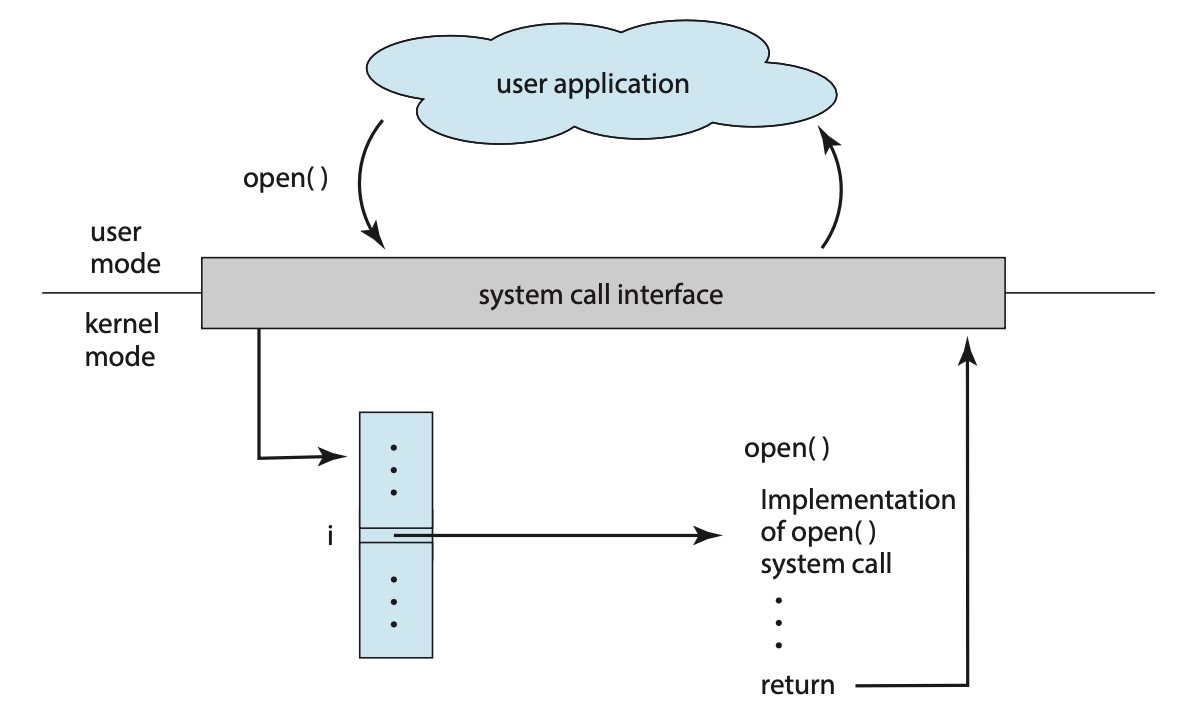
\includegraphics[width=0.65\linewidth]{assets/systemcall.jpg}
    \caption{La gestione della chiamata a sistema \texttt{open()}}
\end{figure}

Spesso è necessario fornire più informazioni della semplice chiamata. Il tipo e la quantità di dati che devono essere forniti alla \textit{system call} possono variare molto.

\spacer
Ci sono diverse soluzioni a questo problema:
\begin{sitemize}
    \item \textbf{Utilizzare i registri}, per quanto sia il metodo più semplice, limita numero e dimensione dei parametri.
    \item Memorizzazione dei parametri su un \textbf{blocco di memoria} e passaggio dell'indirizzo del blocco utilizzando un registro (Linux e Solaris).
    \item \texttt{Push} dei parametri nello \textbf{stack} da parte del programma e poi \textit{}t{pop} da parte del sistema operativo.
\end{sitemize}

\subsection{Application Programming Interface}
Gli sviluppatori spesso non vedono l'implementazione di queste funzioni, che spesso risultano essere estremamente complesse anche per azioni relativamente semplici.

I programmi e i loro sviluppatori interagiscono con delle \textit{Application Programming Interface (API)}, un set di funzioni che sono disponibili al programmatore.

\spacer
L'utilizzo di un'API permette all'utente di non preoccuparsi dei dettagli implementativi e permette una maggiore portabilità del programma ad altri sistemi operativi.

\begin{note}
    Alcune delle API più diffuse ed utilizzate sono la \textit{Win64 API} per Windows, \textit{POSIX API} per Unix, Linux e MacOS e la \textit{Java API} per la \textit{Java Virtual Machine}.
\end{note}

\subsection{Tipologie di Chiamate a Sistema}

Le chiamate a sistema possono essere approssimativamente raggruppate in 6 categorie principali:
\begin{sitemize}
    \item \textbf{Controllo dei Processi:}

    Permette di creare, caricare, eseguire, far attendere e terminare un processo. Inoltre permette di leggere e modificare gli attributi del processo (priorità, tempo di esecuzione, $\ldots$), assegnare/rilasciare memoria e inviare segnali.

    \item \textbf{Gestione delle informazioni:}

    Permette di ottenere informazioni di sistema, la lettura/modifica dell'ora e della data, la lettura/modifica degli attributi di processi, file e dispositivi.

    \item \textbf{Comunicazione:}

    Permette l'apertura/chiusura di una connessione, l'invio/ricezione di messaggi, inserimento/esclusione di dispositivi remoti, condivide informazioni sullo stato dei trasferimenti e gestisce la condivisione della memoria.

    \item \textbf{Gestione dei file:}

    Permette la creazione/eliminazione/apertura/chiusura/lettura/scrittura di file e condivide gli attributi dei file.

    \item \textbf{Gestione dei dispositivi I/O:}

    Permette la richiesta e rilascio di un dispositivo, la lettura e scrittura dei dati e condivide gli attributi di un dispositivo.
\end{sitemize}

\section{Programmi di Sistema}
I programmi di sistema forniscono un ambiente conveniente per lo sviluppo e l'esecuzione di programmi.

In alcuni casi possono essere semplici interfacce per chiamate a sistema, altre volte possono essere più complesse.

\spacer
Alcuni possibili scopi dei programmi di sistema sono:

\begin{sitemize}
    \item \textbf{Gestione di file}
    \item \textbf{Modifica di file}
    \item \textbf{Informazioni di stato}
    \item \textbf{Supporto a linguaggi di programmazione} (compilatori, debugger, $\ldots$)
    \item \textbf{Caricamento ed esecuzione dei programmi}
    \item \textbf{Comunicazioni}
    \item \textbf{Servizi background}

    Sono programmi che vengono lanciati al boot, alcuni terminano dopo aver completato alcune azioni, altri continuano ad essere eseguiti fino allo spegnimento.

    Supportano servizi quali il controllo del disco, scheduling dei processi, logging degli errori, stampa, connessioni di rete, $\ldots$

    \item \textbf{Programmi applicativi}

    Sono Programmi che non fanno parte del sistema operativo (es. browser, editor di testo, $\ldots$), ma sono importanti per l'esperienza degli utenti.
\end{sitemize}

\subsection{Linkers e Loaders}

Dal file sorgente un \textbf{compilatore} crea un file oggetto, il quale è progettato per essere caricato in qualsiasi locazione di memoria.

Poi il \textbf{linker} crea il file eseguibile, combinando i file oggetto e le librerie necessarie.

Il file così generato è pronto per essere caricato in memoria da un \textbf{loader}.

\spacer

I file oggetto ed eseguibili devono avere un formato standard per poter comunicare al sistema operativo come caricare ed eseguire il programma.

Per i sistemi UNIX-like il formato standard è l'\textit{Executable and Linkable Format (ELF)}, per Windows è il formato \textit{PE}, per macOS \textit{Mach-O}.
\begin{figure}[H]
    \centering
    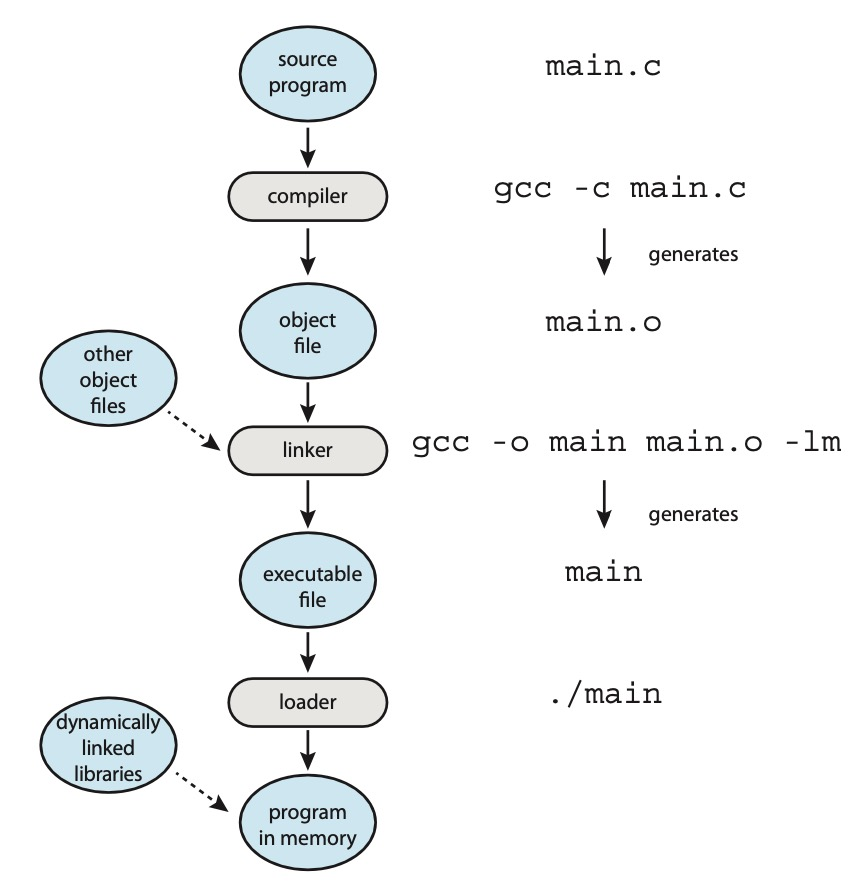
\includegraphics[width=0.38\linewidth]{assets/linker-loader.jpg}
\end{figure}

\begin{note}
    I moderni sistemi operativi \textit{general purpose} non compilano le librerie nei file eseguibili, utilizzano piuttosto delle librerie collegate dinamicamente (es. DLL per Windows) secondo le necessità e condivise da tutti i programmi.
\end{note}

\subsubsection{Le applicazioni sono OS-specific}
Le applicazioni compilate per un sistema \textbf{non} possono, in generale, essere eseguite su altri sistemi. Se questo fosse possibile non dovremmo scegliere il sistema operativo in base agli applicativi che sono disponibili, ma in base alle funzionalità del sistema.

\spacer
Parte del problema, che rende difficile l'interoperabilità tra sistemi, è che ognuno ha il suo \textbf{set di chiamate} a sistema, i propri formati di file eseguibili, ...

\spacer
Ci sono alcune soluzioni per scrivere codice che può essere eseguito su più sistemi:
\begin{itemize}
    \item Scrivere in un \textbf{linguaggio interpretato}, come Python, in questo caso è sufficiente che esista un interprete disponibile per quel sistema operativo.

    \item Scrivere in un linguaggio che \textbf{include una VM} all'interno della quale avviene l'esecuzione, come Java.

    \item Scrivere in un \textbf{linguaggio standard}, come C, e compilare poi per ogni sistema.
\end{itemize}

\subsubsection{ABI}
Proprio come le API permettono al programmatore di non dover programmare le implementazioni di semplici funzioni in codice macchina, le ABI forniscono al compilatore il set di istruzioni che possono essere eseguite sulla specifica architettura per cui si sta compilando.

\spacer
Il problema è che le ABI spesso non forniscono una gran quantità di interoperabilità, quindi il codice deve essere compilato \textbf{per ogni sistema operativo} e \textbf{per ogni architettura} su cui verrà eseguito.

\section{Implementazione di un Sistema Operativo}

Tradizionalmente i sistemi operativi venivano scritti in assembly, successivamente vennero utilizzati dei linguaggi specifici e ad oggi si utilizza principalmente C o C++ per scrivere il \textit{kernel}, assieme a frammenti in assembly per gli elementi di basso livello.

\spacer
Vista la complessità del codice richiesto da un sistema operativo è importante pensare alla struttura da impartire ad esso, vediamo ora le strutture più comune che vengono usate per la creazione dei sistemi operativi.

\begin{figure}[H]
    \centering
    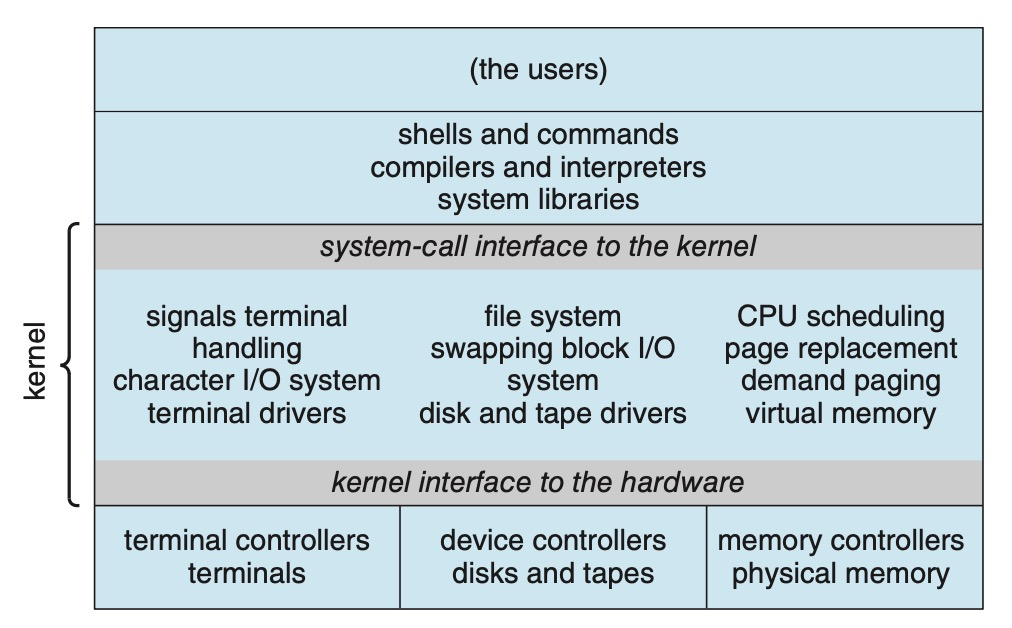
\includegraphics[width=0.55\linewidth]{assets/os-structure.jpg}
\end{figure}

\subsection{Design di un Sistema Operativo}
Abbiamo già visto come vengono definiti gli obiettivi del sistema operativo, vedendo cosa gli utenti e l'hardware si aspettano da esso.

\spacer

Nella progettazione di un software complesso come il sistema operativo è importante mantenere separati i due concetti di politiche e meccanismi.

Le \textbf{politiche} definiscono i compiti e servizi che il sistema operativo deve fornire, mentre i \textbf{meccanismi} definiscono come queste politiche andranno implementate all'atto pratico.

\begin{note}
    In macos e Windows politiche e meccanismi sono fissati a priori e scritti nel sistema, in Linux la separazione tra le due è più evidente.
\end{note}

\subsection{Monolitici}
La struttura più semplice è l'\textbf{assenza di una struttura}. Tutta la funzionalità del kernel viene implementata in un unico eseguibile, con tutte le funzioni strettamente collegate.

\spacer
Questo significa che un singolo bug in uno dei sistemi può comportare il blocco dell'intero sistema, inoltre lo sviluppo e l'estensione risultano essere particolarmente complicati per un kernel monolitico.

Tuttavia quando costruito in modo sicuro la stretta integrazione rende il sistema \textbf{estremamente efficiente}.

\begin{note}
    MS-DOS non implementava una struttura modulare, le applicazioni fanno chiamate a system call direttamente, aprendo così la strada a diverse vulnerabilità.

    \spacer
    Anche UNIX implementava un kernel parzialmente monolitico, con l'obiettivo di migliorare le performance.
    Esso presentava solo due livelli, il kernel e le applicazioni utente. Lo strato del kernel si ritrova con una gran quantità di responsabilità.

    \begin{figure}[H]
        \centering
        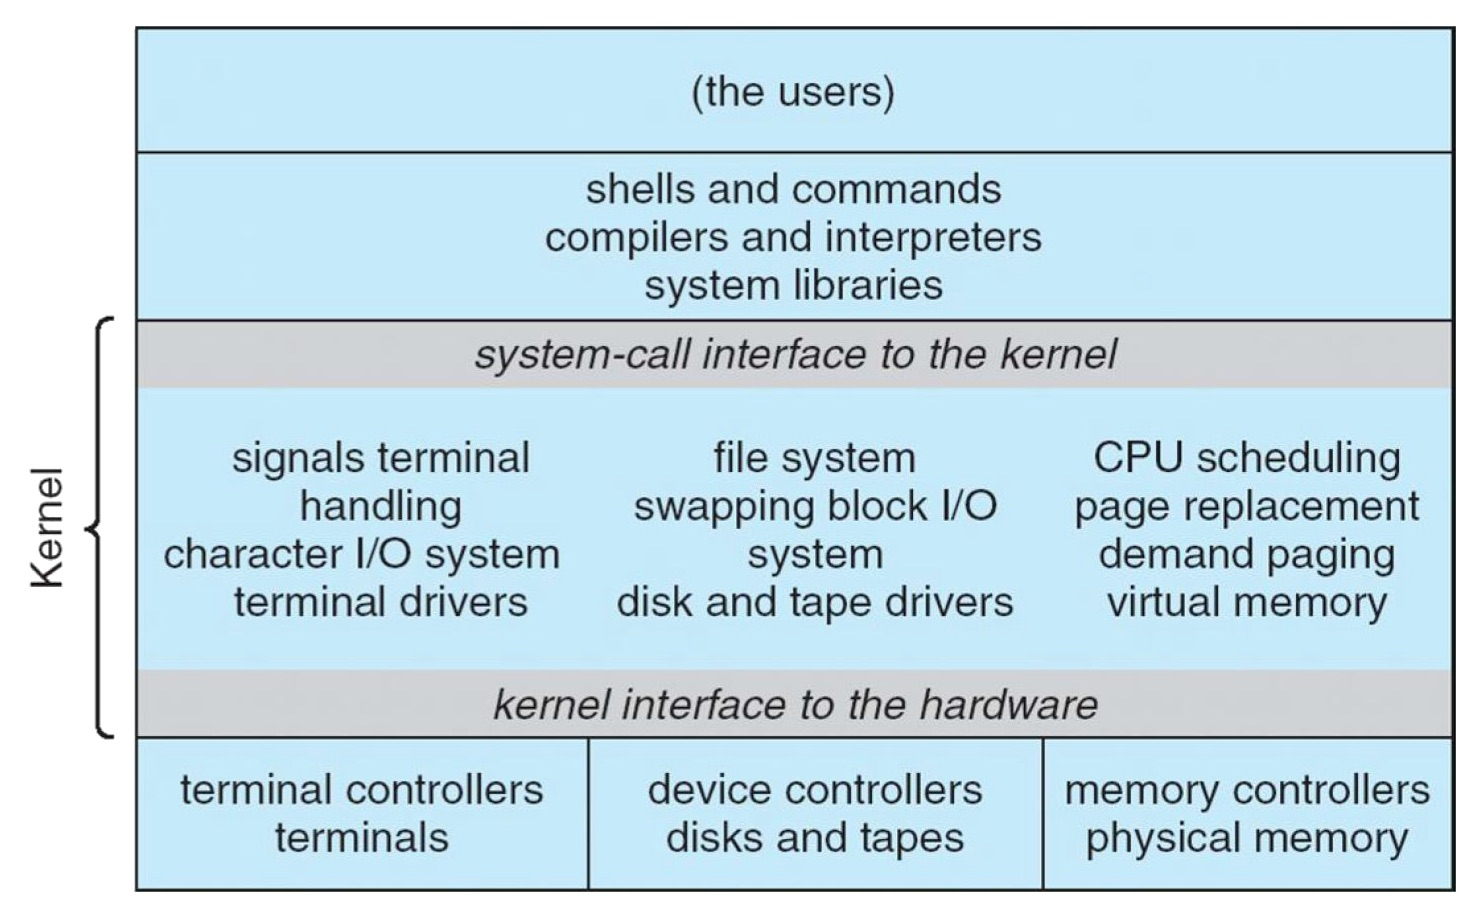
\includegraphics[width=0.5\linewidth]{assets/unix-monolithic.jpeg}
    \end{figure}
\end{note}

\subsection{Approccio stratificato}
L'alternativa all'approccio monolitico è un approccio dove i vari sistemi sono separati in componenti o moduli relativamente piccoli che assieme compongono il kernel.

\spacer
Uno dei modi per implementare un approccio modulare è quello stratificato, in presenza di hardware appropriato è possibile suddividere le funzioni del sistema operativo su vari \textbf{livelli}. Il livello 0 è l'hardware, il livello N è l'interfaccia utente.

Ciascuno strato impiega esclusivamente funzioni degli strati di livello inferiore.

\spacer
Questa struttura ha il vantaggio di facilitare la realizzazione e messa a punto del sistema operativo.

Gli svantaggi invece sono legati ai tempi di attraversamento dei vari strati (si pensi ad una system call che deve essere intercettata e riportata da molteplici livelli) e alla difficoltà di definire gli strati, in quanto essi possono usare solo le funzioni degli strati inferiori (si pensi al driver della memoria virtuale, che dovrebbe essere sopra allo scheduler, perché deve essere possibile interromperne l'esecuzione in caso di page fault. Ma allo stesso tempo lo scheduler deve essere a conoscenza delle informazioni del driver per poter gestire al meglio i processi).

\begin{figure}[H]
    \centering
    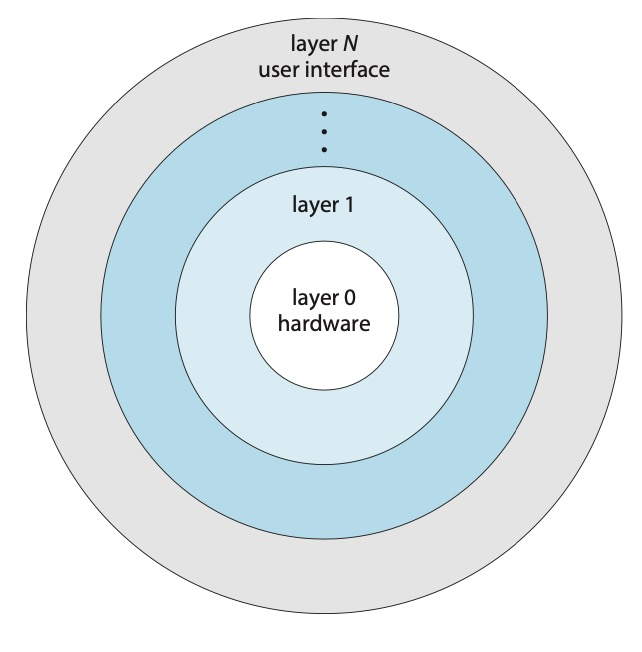
\includegraphics[width=0.4\linewidth]{assets/os-layered.jpg}
\end{figure}

\subsection{Microkernel}
Un microkernel offre la \textbf{minima quantità di servizi} di gestione dei processi, della memoria e di comunicazione.

Tutte le funzionalità non essenziali al kernel sono implementate come programmi utente, c'è quindi necessità di intensa comunicazione tra le varie componenti, cosa che viene mediata dal kernel.

\spacer
Il microkernel è semplice da modificare e rende semplice aggiungere e modificare le funzionalità, in quanto esse sono implementate a livello utente.

Inoltre i sistemi operativi con microkernel sono più sicuri (meno codice viene eseguito a livello kernel) e sono più facili da portare a nuove architetture.

Il più grande svantaggio è l'\textbf{overhead} di prestazioni causato dalle continue comunicazioni tra i moduli.

\begin{figure}[H]
    \centering
    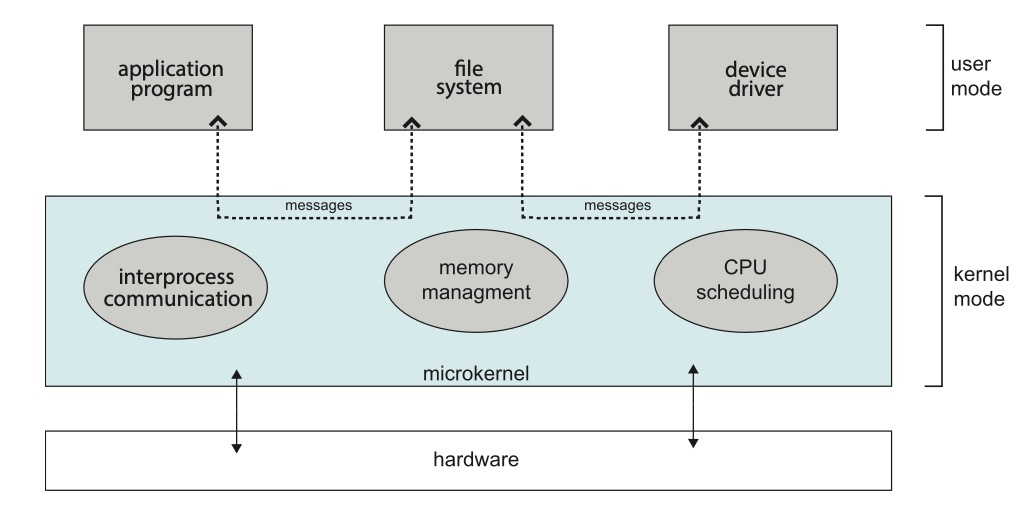
\includegraphics[width=0.5\linewidth]{assets/microkernel.jpg}
\end{figure}

\begin{note}
    Utilizzato da alcuni sistemi operativi più vecchi, come le prime versioni di Windows NT o macOS su kernel darwin.
\end{note}

\subsection{Kernel Modulari}
L'implementazione di tutti i moderni sistemi operativi utilizza i \textit{Loadable Kernel Module (LKMs)}.
Si utilizza un approccio object-oriented dove ciascun modulo implementa un'interfaccia che definisce una funzione del kernel.

Ciascun modulo può comunicare con gli altri moduli mediante l'interfaccia comune, inoltre ogni modulo può essere caricato o meno in memoria in base alle necessità.

\spacer
Questo approccio è simile a quello del microkernel con solo alcuni moduli caricati inizialmente che hanno il compito di caricare gli altri in base alla necessità, ma vengono risolti i problemi di comunicazione.

\subsection{Sistemi ibridi}
Nei sistemi operativi moderni si utilizza spesso un approccio misto rispetto a quelli visti precedentemente.

\subsubsection*{Linux}
Linux ha un kernel principalmente monolitico per poter fornire prestazioni elevate, tuttavia esso può essere anche esteso in modo dinamico.

\subsubsection*{Windows}
Anche Windows è in larga parte monolitico, ma conserva alcune caratteristiche tipiche dei sistemi microkernel tramite il supporto per sottosistemi (\textit{personalities}) che vengono eseguiti a livello utente.

\subsubsection*{macOS e iOS}
Anche se i sistemi possono sembrare molto differenti e vengono eseguiti su architetture e dispositivi diversi, essi condividono una struttura simile.

\spacer
\begin{sitemize}
    \item \textbf{User experience (GUI):} Permette l'interazione col software, diversa per macOS e iOS in base allo stile di input.
    \item \textbf{Ambienti applicativi:} Cocoa fornisce le API per i linguaggi di programmazione Objective-C e Swift.
    \item \textbf{Framework di base:} Ambienti che supportano le API grafiche e di base, come OpenGL.
    \item \textbf{Ambiente kernel:} Darwin include il kernel BSD UNIX, è estendibile grazie ai kext utili allo sviluppo di driver ed estensioni del kernel.
\end{sitemize}
\spacer

Le applicazioni su questi sistemi possono essere progettate per sfruttare le funzionalità di user experience o per aggirarle completamente (disponibile ai developer solo su macOS).

\begin{figure}[H]
    \centering
    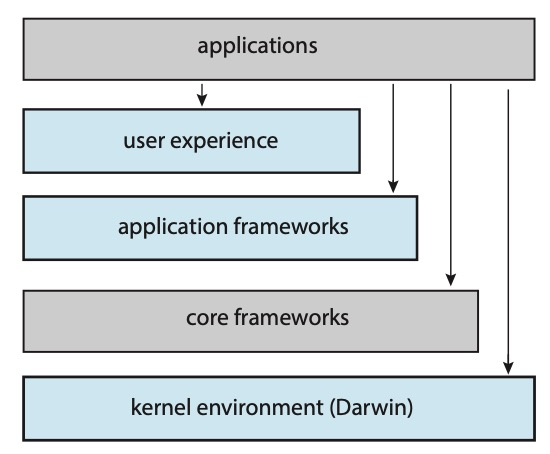
\includegraphics[width=0.4\linewidth]{assets/apple-os-structure.jpg}
    \caption{Struttura dei sistemi macOS e iOS}
\end{figure}

\subsubsection*{Android}
Sviluppato dalla \textit{Open Headset Alliance} di cui Google fa parte, ma non è l'unica grande azienda, Android è un sistema operativo open source che gestisce una gran quantità di dispositivi mobili.

\spacer

Android nasce da una versione modificata del kernel linux, le applicazioni android sono scritte in Java e vengono poi eseguite sull'\textit{Android RunTime (ART)}.
Per migliorare le prestazioni ART non esegue una compilazione a tempo di esecuzione, ma viene eseguita all'installazione dell'applicazione.

Gli sviluppatori possono anche scegliere di utilizzare JNI, l'interfaccia nativa con un accesso più diretto all'hardware.

\begin{figure}[H]
    \centering
    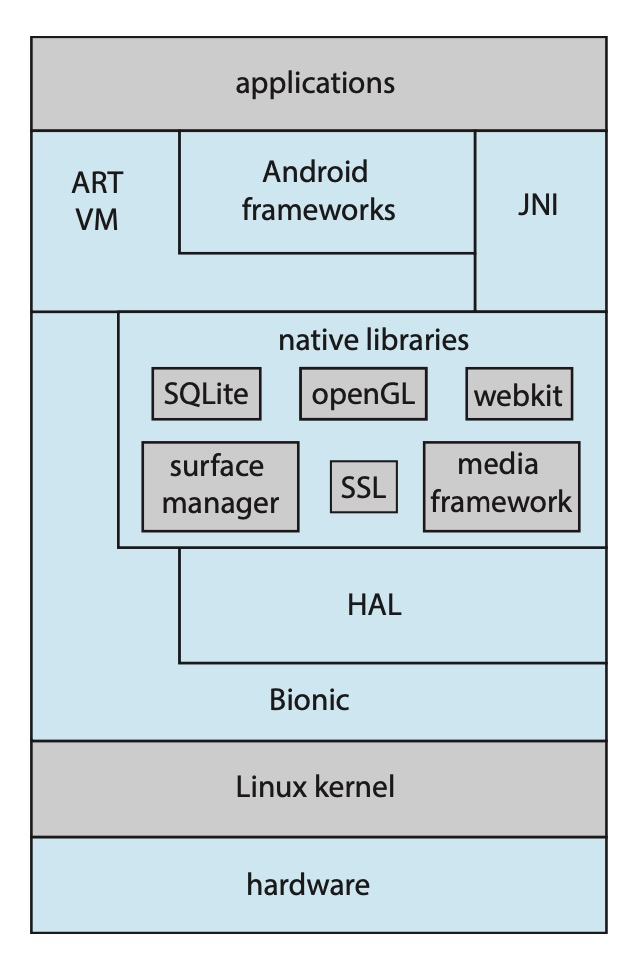
\includegraphics[width=0.27\linewidth]{assets/android.jpg}
    \caption{Struttura sistema android}
\end{figure}

\begin{note}
    Poiché i dispositivi android hanno specifiche hardware pressoché illimitato c'è un livello di astrazione tra l'hardware e le librerie native (\textit{Hardware Abstraction Layer, HAL})
\end{note}

\section{Debugging e Tuning}
Il \textbf{debugging} è l'attività di individuazione e risoluzione dei problemi, il che comprende sia la risoluzione dei bug che il performance tuning.

\spacer
Il sistema operativo aiuta nel processo con la generazione di \textbf{file di log} che danno informazioni sugli errori rilevati durante l'esecuzione.
Inoltre il sistema operativo fornisce un \textbf{core dump}, ovvero una copia della memoria impiegata dal processo al momento della terminazione anomala.

\begin{note}
    \textbf{Kernel}

    Quando avviene un errore al kernel viene chiamato \textbf{crash}. Quando questo avviene viene creato un \textbf{crash dump} che viene inserito in un'apposita sezione della memoria.

    \spacer
    È necessario di scrivere su un'area riservata di memoria perché quando si ottiene un crash lo stato del sistema non è garantito ed è difficile comprendere quali sezioni della memoria sono libere.
\end{note}

\subsection{Tuning}
Anche i problemi che condizionano le prestazioni sono considerati bachi e vanno quindi trovati e risolti.
Il performance tuning è l'insieme delle tecniche atte ad ottimizzare le prestazioni del sistema ed ad eliminare i colli di bottiglia.

\spacer
Per fare ciò ci sono varie tecniche, è possibile eseguire del codice che misuri le prestazioni del sistema e poi ne salvi i risultati su un file di log.

Oppure possono essere utilizzati degli strumenti grafici del sistema operativo, ad es. task manager di Windows.

Infine esiste anche il profiling che punta a visualizzare quali chiamate a sistema vengono utilizzare maggiormente così da ottimizzarle, quando possibile.